\documentclass[tikz,crop,convert={density=200,outext=.png},border=0.0cm]{standalone}

\usepackage{amsmath}
\usepackage{physics}
\usepackage{graphicx}
\usepackage{xcolor}

\definecolor{boundary_hole}{RGB}{103,0,31} % Dark magenta
\definecolor{hole}{RGB}{255,247,251} % Extremely light blue (almost white)
\definecolor{adjacent}{RGB}{116,169,207} % Medium blue
\definecolor{rest}{RGB}{2,56,88} % Dark blue

\begin{document}
\begin{tikzpicture}
\node[inner sep=0pt] (mesh) at (0,0)
{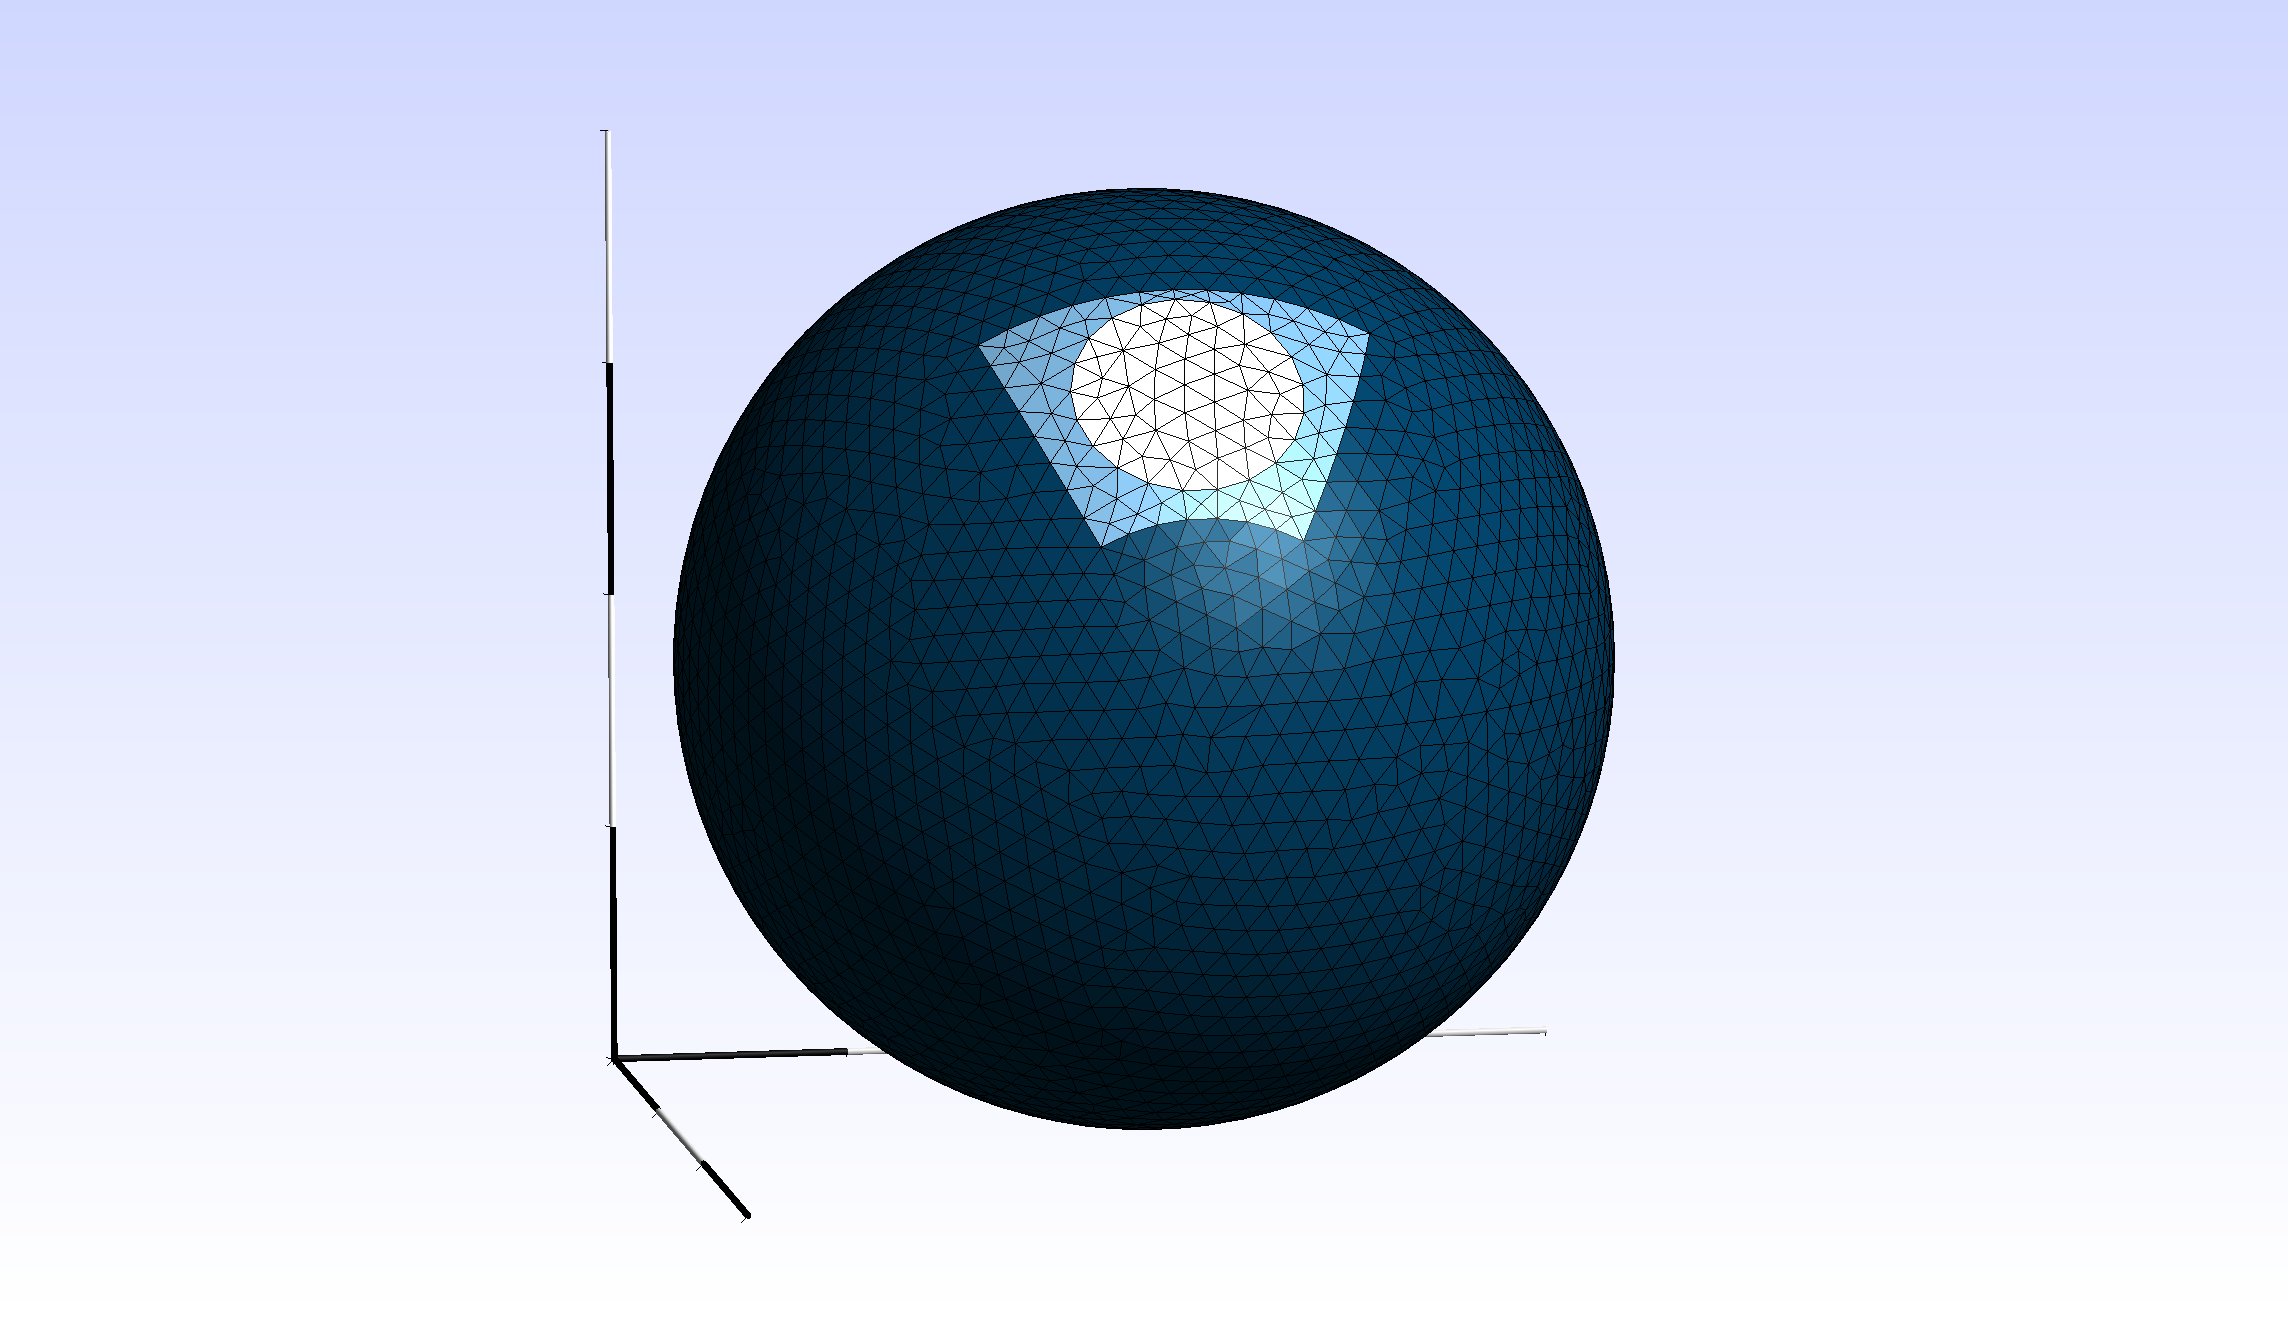
\includegraphics[scale=0.5]{test_2.png}};
% \fill[blue!40!white] (0,0) rectangle (4,4);
%\node[rectangle,draw,fill=boundary_hole,minimum size=2cm] (r) at (15.2,8) {\huge \color{white}The boundary of the hole $\Gamma$};
%\node[rectangle,draw,fill=hole,minimum size=2cm] (r) at (15.2,6) {\huge \color{black}Hole\;\;\;\;\;\;\;\;\;\;\;\;\;\;\;\;\;\;\;\;\;\;\;\;\;\;\;\;\;\;\;\;\;\;\;\;\,};
\node[rectangle,draw,fill=hole,minimum size=2cm] (r) at (15.2,6) {\huge \color{black}Budscar\;\;\;\;\;\;\;\;\;\;\;\;\;\;\;\;\;\;\;\;\;\;\;\;\;\;\;\;\;\;\;};
\node[rectangle,draw,fill=adjacent,minimum size=2cm] (r) at (15.2,2)
{\huge \color{white}Adjacent region $\Omega_2$\;\;\;\;\;\;\;\;\;\;\;\;\;\,};
\node[rectangle,draw,fill=rest,,minimum size=2cm] (r) at (15.2,4) {\huge \color{white}The sphere $\Omega_1$\;\;\;\;\;\;\;\;\;\;\;\;\;\;\;\;\;\;\;\;\;};
\end{tikzpicture}

\end{document}
